A ViT-B-16 iteratív tanításának eredményei négy lépésben először 1000 majd 5000 azután 10000 végül pedig 25000 képes halmazon. Ezelet a lépéseket 1k, 5k 10k 25k rövidítésekkel fogom jelölni.

%1K-----------------------------------------------------------------------------
\subsubsection{1k adathalmazon történő tanítás lépései ViT-B-16 modellen.}
  \begin{itemize} 
    \item Epoch 1/10 - train: 15/15 [00:07<00:00, 2.05it/s]
    \item Epoch 1: Train loss=4.6843, acc=0.0417 Val loss=3.8488, acc=0.2340
    \item Epoch 2/10 - train: 15/15 [00:06<00:00, 2.36it/s]
    \item Epoch 2: Train loss=2.5164, acc=0.4397 Val loss=2.8448, acc=0.3132
    \item Epoch 3/10 - train: 15/15 [00:06<00:00, 2.36it/s]
    \item Epoch 3: Train loss=0.5900, acc=0.8640 Val loss=2.9254, acc=0.3244
    \item Epoch 4/10 - train: 15/15 [00:06<00:00, 2.36it/s]
    \item Epoch 4: Train loss=0.1434, acc=0.9693 Val loss=2.7853, acc=0.3690
    \item Epoch 5/10 - train: 15/15 [00:06<00:00, 2.36it/s]
    \item Epoch 5: Train loss=0.0588, acc=0.9879 Val loss=2.9444, acc=0.3470
    \item Epoch 6/10 - train: 15/15 [00:06<00:00, 2.36it/s]
    \item Epoch 6: Train loss=0.0383, acc=0.9923 Val loss=2.8805, acc=0.3618
    \item Epoch 7/10 - train: 15/15 [00:06<00:00, 2.36it/s]
    \item Epoch 7: Train loss=0.0187, acc=0.9967 Val loss=2.9450, acc=0.3536
    \item Epoch 8/10 - train: 15/15 [00:06<00:00, 2.36it/s]
    \item Epoch 8: Train loss=0.0146, acc=0.9956 Val loss=2.8890, acc=0.3685
    \item Epoch 9/10 - train: 15/15 [00:06<00:00, 2.36it/s]
    \item Epoch 9: Train loss=0.0106, acc=0.9967 Val loss=2.9405, acc=0.3596
    \item Epoch 10/10 - train: 15/15 [00:06<00:00, 2.36it/s]
    \item Epoch 10: Train loss=0.0052, acc=0.9989 Val loss=2.9333, acc=0.3622
  \end{itemize}

\subsubsection{1k adathalmazon történő tanítás grafikonja ViT-B-16 modellen.}
  \begin{figure}[H]
    \centering
    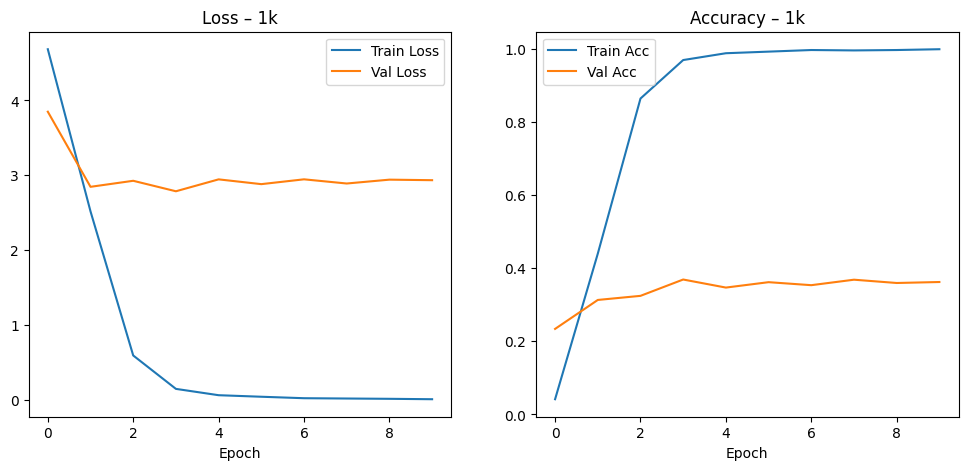
\includegraphics[width=1.0\textwidth]{images/phase03/phase03_ViT-B-16_1K_learning_curve.png}
    \caption{1k adathalmazon történő tanítás grafikonja ViT-B-16 modellen.}
    \label{fig:phase03_ViT-B-16_1K_learning_curve}
  \end{figure}

  \subsubsection{1k adathalmazon történő tanítás eredményei.}
    \begin{center}
      \begin{longtable}{l c}
      \caption{1k tanítás ViT-B-16-en.} \label{tab:phase03_ViT-B-16_1k} \\
      \toprule
      \textbf{Metrika} & \textbf{Érték} \\
      \midrule
      \endfirsthead
      \toprule
      \textbf{Metrika} & \textbf{Érték} \\
      \midrule
      \endhead
      Top-1 Accuracy & 0.3645 \\
      Top-5 Accuracy & 0.6646 \\
      Precision      & 0.3144 \\
      Recall         & 0.3529 \\
      F1-score       & 0.3138 \\
      Inference time & 41.85 sec \\
      \bottomrule
      \end{longtable}
    \end{center}

%5K-----------------------------------------------------------------------------
\subsubsection{5k adathalmazon történő tanítás lépései ViT-B-16 modellen.}
  \begin{itemize} 
    \item Epoch 1/10 - train: 77/77 [00:32<00:00, 2.34it/s]
    \item Epoch 1: Train loss=3.3736, acc=0.2326 Val loss=1.9799, acc=0.4640
    \item Epoch 2/10 - train: 77/77 [00:32<00:00, 2.34it/s]
    \item Epoch 2: Train loss=1.3933, acc=0.6246 Val loss=2.2583, acc=0.4311
    \item Epoch 3/10 - train: 77/77 [00:32<00:00, 2.34it/s]
    \item Epoch 3: Train loss=0.4573, acc=0.8621 Val loss=2.3891, acc=0.4585
    \item Epoch 4/10 - train: 77/77 [00:32<00:00, 2.34it/s]
    \item Epoch 4: Train loss=0.1984, acc=0.9466 Val loss=2.5042, acc=0.4547
    \item Epoch 5/10 - train: 77/77 [00:32<00:00, 2.34it/s]
    \item Epoch 5: Train loss=0.1027, acc=0.9735 Val loss=2.4770, acc=0.4799
    \item Epoch 6/10 - train: 77/77 [00:32<00:00, 2.34it/s]
    \item Epoch 6: Train loss=0.0585, acc=0.9849 Val loss=2.7746, acc=0.4417
    \item Epoch 7/10 - train: 77/77 [00:32<00:00, 2.34it/s]
    \item Epoch 7: Train loss=0.0399, acc=0.9900 Val loss=2.4442, acc=0.4971
    \item Epoch 8/10 - train: 77/77 [00:32<00:00, 2.34it/s]
    \item Epoch 8: Train loss=0.0367, acc=0.9916 Val loss=2.6809, acc=0.4699
    \item Epoch 9/10 - train: 77/77 [00:32<00:00, 2.34it/s]
    \item Epoch 9: Train loss=0.0757, acc=0.9814 Val loss=2.6012, acc=0.4806
    \item Epoch 10/10 - train: 77/77 [00:32<00:00, 2.34it/s]
    \item Epoch 10: Train loss=0.0750, acc=0.9816 Val loss=2.9607, acc=0.4482
  \end{itemize}

\subsubsection{5k adathalmazon történő tanítás grafikonja ViT-B-16 modellen.}
  \begin{figure}[H]
    \centering
    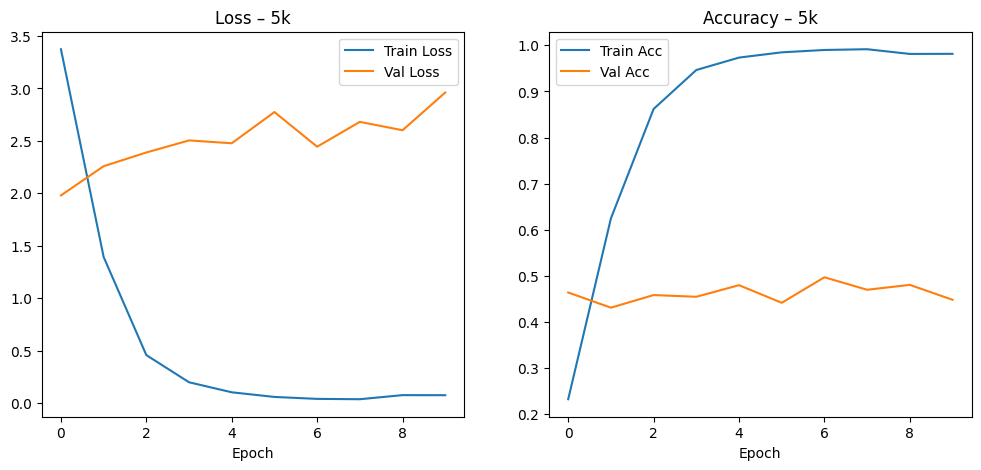
\includegraphics[width=1.0\textwidth]{images/phase03/phase03_ViT-B-16_5K_learning_curve.png}
    \caption{5k adathalmazon történő tanítás grafikonja ViT-B-16 modellen.}
    \label{fig:phase03_ViT-B-16_5K_learning_curve}
  \end{figure}

\subsubsection{5k adathalmazon történő tanítás eredményei.}
  \begin{center}
    \begin{longtable}{l c}
    \caption{5k tanítás ViT-B-16-en.} \label{tab:phase03_ViT-B-16_5k} \\
    \toprule
    \textbf{Metrika} & \textbf{Érték} \\
    \midrule
    \endfirsthead
    \toprule
    \textbf{Metrika} & \textbf{Érték} \\
    \midrule
    \endhead
    Top-1 Accuracy & 0.4482 \\
    Top-5 Accuracy & 0.7332 \\
    Precision      & 0.4442 \\
    Recall         & 0.4805 \\
    F1-score       & 0.4364 \\
    Inference time & 41.93 sec \\
    \bottomrule
    \end{longtable}
  \end{center}

%10K-----------------------------------------------------------------------------
\subsubsection{10k adathalmazon történő tanítás lépései ViT-B-16 modellen.}
  \begin{itemize} 
    \item Epoch 1/10 - train: 155/155 [01:06<00:00, 2.34it/s]
    \item Epoch 1: Train loss=2.5420, acc=0.3893 Val loss=1.9267, acc=0.4716
    \item Epoch 2/10 - train: 155/155 [01:06<00:00, 2.34it/s]
    \item Epoch 2: Train loss=1.0743, acc=0.6928 Val loss=1.8801, acc=0.5144
    \item Epoch 3/10 - train: 155/155 [01:06<00:00, 2.34it/s]
    \item Epoch 3: Train loss=0.4640, acc=0.8644 Val loss=2.2153, acc=0.4892
    \item Epoch 4/10 - train: 155/155 [01:06<00:00, 2.34it/s]
    \item Epoch 4: Train loss=0.2552, acc=0.9249 Val loss=2.2827, acc=0.5049
    \item Epoch 5/10 - train: 155/155 [01:06<00:00, 2.34it/s]
    \item Epoch 5: Train loss=0.1651, acc=0.9544 Val loss=2.4475, acc=0.5005
    \item Epoch 6/10 - train: 155/155 [01:06<00:00, 2.34it/s]
    \item Epoch 6: Train loss=0.1221, acc=0.9686 Val loss=2.5930, acc=0.4947
    \item Epoch 7/10 - train: 155/155 [01:06<00:00, 2.34it/s]
    \item Epoch 7: Train loss=0.1071, acc=0.9717 Val loss=2.5967, acc=0.5050
    \item Epoch 8/10 - train: 155/155 [01:06<00:00, 2.34it/s]
    \item Epoch 8: Train loss=0.1029, acc=0.9707 Val loss=2.7910, acc=0.4855
    \item Epoch 9/10 - train: 155/155 [01:06<00:00, 2.34it/s]
    \item Epoch 9: Train loss=0.1593, acc=0.9533 Val loss=2.9414, acc=0.4619
    \item Epoch 10/10 - train: 155/155 [01:06<00:00, 2.34it/s]
    \item Epoch 10: Train loss=0.1899, acc=0.9463 Val loss=2.9566, acc=0.4733
  \end{itemize}

\subsubsection{10k adathalmazon történő tanítás grafikonja ViT-B-16 modellen.}
  \begin{figure}[H]
    \centering
    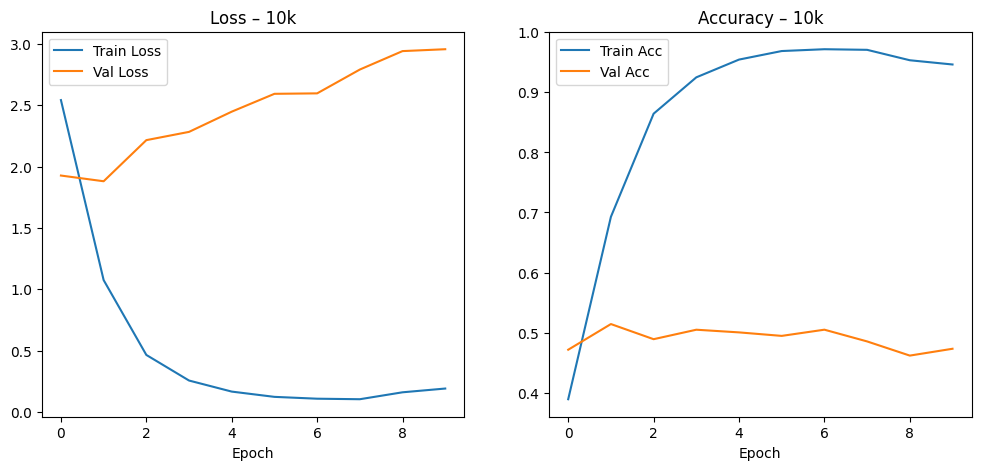
\includegraphics[width=1.0\textwidth]{images/phase03/phase03_ViT-B-16_10K_learning_curve.png}
    \caption{10k adathalmazon történő tanítás grafikonja ViT-B-16 modellen.}
    \label{fig:phase03_ViT-B-16_10K_learning_curve}
  \end{figure}

\subsubsection{10k adathalmazon történő tanítás eredményei.}
  \begin{center}
    \begin{longtable}{l c}
    \caption{10k tanítás ViT-B-16-en.} \label{tab:phase03_ViT-B-16_10k} \\
    \toprule
    \textbf{Metrika} & \textbf{Érték} \\
    \midrule
    \endfirsthead
    \toprule
    \textbf{Metrika} & \textbf{Érték} \\
    \midrule
    \endhead
    Top-1 Accuracy & 0.4782 \\
    Top-5 Accuracy & 0.7643 \\
    Precision      & 0.4558 \\
    Recall         & 0.5071 \\
    F1-score       & 0.4540 \\
    Inference time & 41.93 sec \\
    \bottomrule
    \end{longtable}
  \end{center}

%25K-----------------------------------------------------------------------------
\subsubsection{25k adathalmazon történő tanítás lépései ViT-B-16 modellen.}
  \begin{itemize} 
    \item Epoch 1/10 - train: 391/391 [02:46<00:00, 2.35it/s]
    \item Epoch 1: Train loss=2.0880, acc=0.4653 Val loss=1.6953, acc=0.5265
    \item Epoch 2/10 - train: 391/391 [02:46<00:00, 2.35it/s]
    \item Epoch 2: Train loss=1.0699, acc=0.6904 Val loss=1.7175, acc=0.5424
    \item Epoch 3/10 - train: 391/391 [02:46<00:00, 2.35it/s]
    \item Epoch 3: Train loss=0.6086, acc=0.8187 Val loss=1.8424, acc=0.5568
    \item Epoch 4/10 - train: 391/391 [02:46<00:00, 2.35it/s]
    \item Epoch 4: Train loss=0.3954, acc=0.8805 Val loss=2.5127, acc=0.5002
    \item Epoch 5/10 - train: 391/391 [02:46<00:00, 2.35it/s]
    \item Epoch 5: Train loss=0.2781, acc=0.9177 Val loss=2.1648, acc=0.5591
    \item Epoch 6/10 - train: 391/391 [02:46<00:00, 2.35it/s]
    \item Epoch 6: Train loss=0.2536, acc=0.9223 Val loss=2.3969, acc=0.5246
    \item Epoch 7/10 - train: 391/391 [02:46<00:00, 2.35it/s]
    \item Epoch 7: Train loss=0.2210, acc=0.9349 Val loss=2.4331, acc=0.5260
    \item Epoch 8/10 - train: 391/391 [02:46<00:00, 2.35it/s]
    \item Epoch 8: Train loss=0.1903, acc=0.9439 Val loss=2.4245, acc=0.5370
    \item Epoch 9/10 - train: 391/391 [02:46<00:00, 2.35it/s]
    \item Epoch 9: Train loss=0.1684, acc=0.9512 Val loss=2.7019, acc=0.5152
    \item Epoch 10/10 - train: 391/391 [02:46<00:00, 2.35it/s]
    \item Epoch 10: Train loss=0.1742, acc=0.9479 Val loss=2.7032, acc=0.5316
  \end{itemize}

\subsubsection{25k adathalmazon történő tanítás grafikonja ViT-B-16 modellen.}
  \begin{figure}[H]
    \centering
    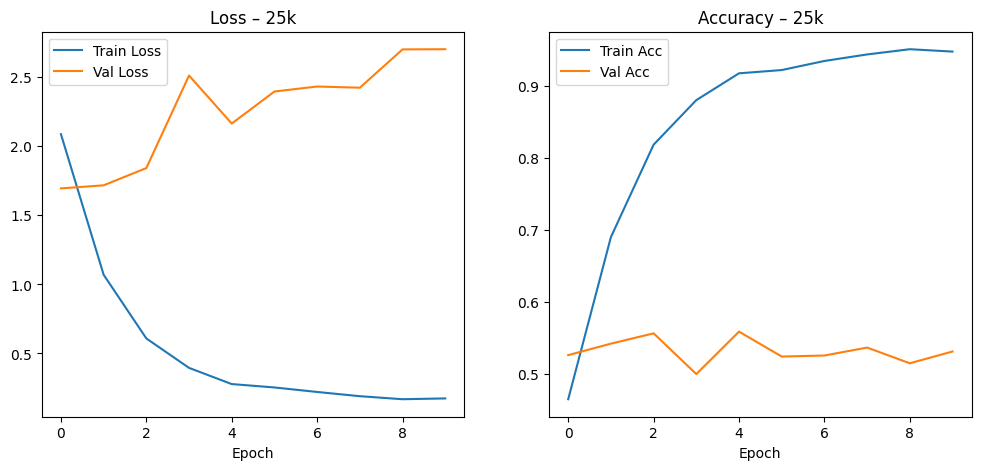
\includegraphics[width=1.0\textwidth]{images/phase03/phase03_ViT-B-16_25K_learning_curve.png}
    \caption{25k adathalmazon történő tanítás grafikonja ViT-B-16 modellen.}
    \label{fig:phase03_ViT-B-16_25K_learning_curve}
  \end{figure}

\subsubsection{25k adathalmazon történő tanítás eredményei.}
  \begin{center}
    \begin{longtable}{l c}
    \caption{25k tanítás ViT-B-16-en.} \label{tab:phase03_ViT-B-16_25k} \\
    \toprule
    \textbf{Metrika} & \textbf{Érték} \\
    \midrule
    \endfirsthead
    \toprule
    \textbf{Metrika} & \textbf{Érték} \\
    \midrule
    \endhead
    Top-1 Accuracy & 0.5335 \\
    Top-5 Accuracy & 0.8185 \\
    Precision      & 0.5189 \\
    Recall         & 0.5908 \\
    F1-score       & 0.5308 \\
    Inference time & 42.08 sec \\
    \bottomrule
    \end{longtable}
  \end{center}

\subsubsection{ViT-B-16 iteratív tanítás összefoglaló}
  \begin{center}
    \begin{longtable}{lllllll}
    \caption{Összehasonlító táblázat a ViT-B-16 iteratív tanításáról.}\label{tab:phase3_ViT-B-16_summary_table}\\
    \toprule
    Minta & Top-1 & Top-5 & Precision & Recall & F1 & Time(s) \\
    \midrule
    \endfirsthead
    \toprule
    Minta & Top-1 & Top-5 & Precision & Recall & F1 & Time(s) \\
    \midrule
    \endhead
    1k & 0.3645 & 0.6646 & 0.3144 & 0.3529 & 0.3138 & 41.85 \\
    5k & 0.4482 & 0.7332 & 0.4442 & 0.4805 & 0.4364 & 41.93 \\
    10k & 0.4782 & 0.7643 & 0.4558 & 0.5071 & 0.4540 & 41.93 \\
    25k & 0.5335 & 0.8185 & 0.5189 & 0.5908 & 0.5308 & 42.08 \\
    \bottomrule
    \end{longtable}
  \end{center}

  \subsubsection{Összehasonlító grafikon a ViT-B-16 iteratív tanításáról.}
  \begin{figure}[H]
    \centering
    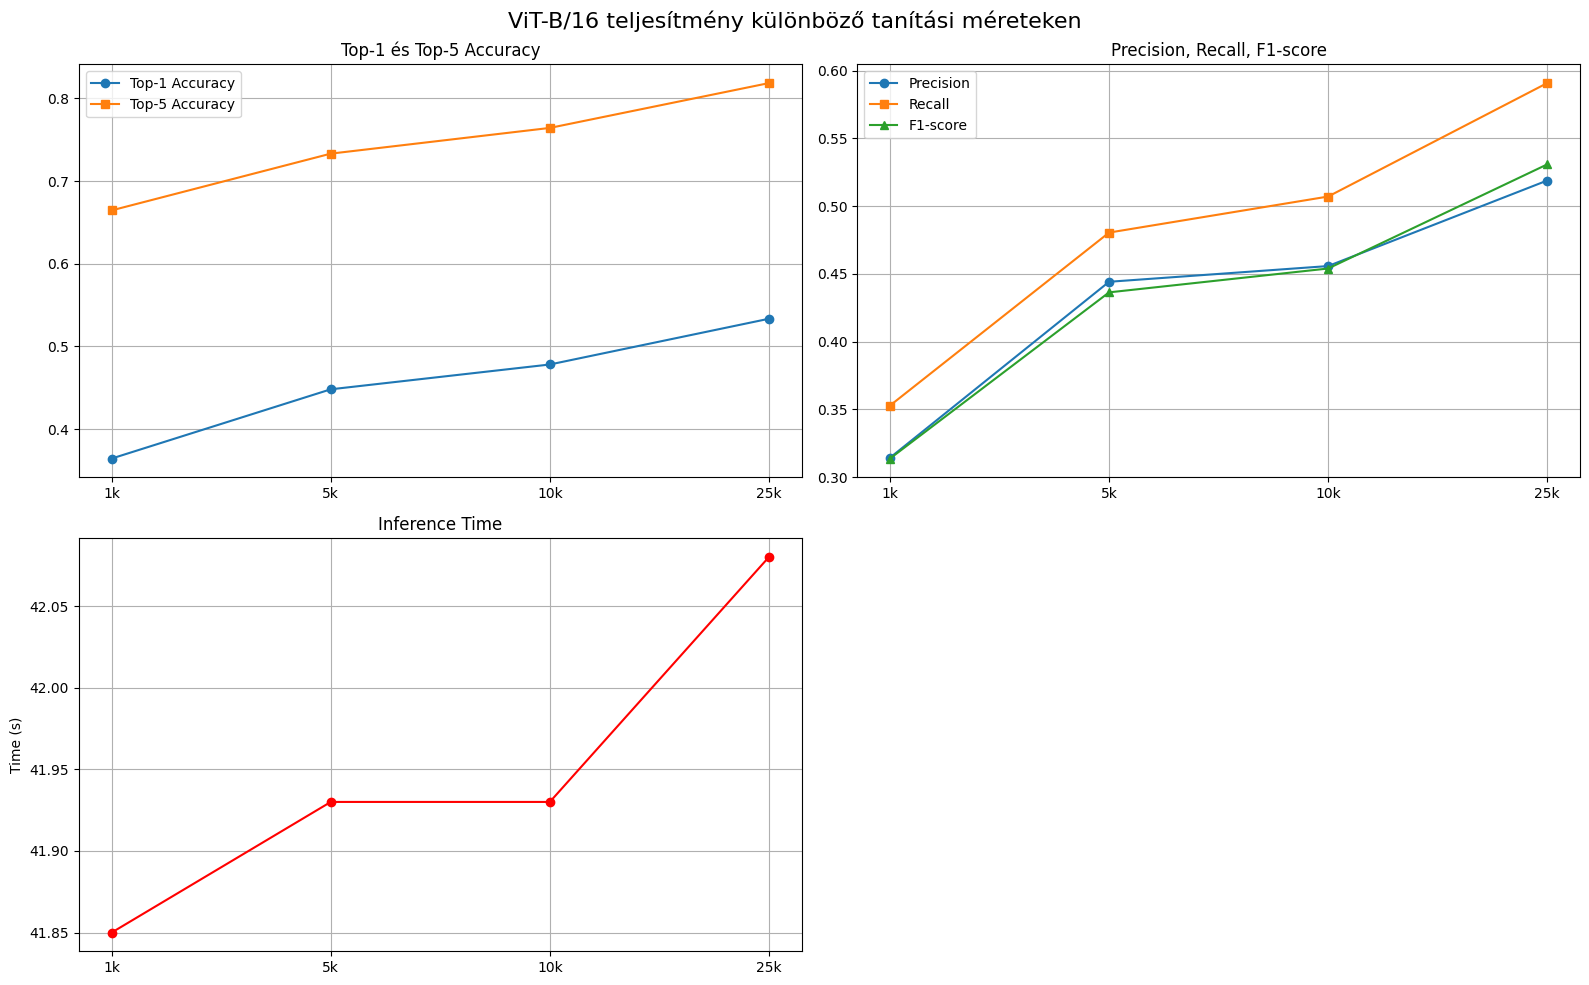
\includegraphics[width=1.0\textwidth]{images/phase03/phase03_ViT-B-16_summary_curve.png}
    \caption{Összehasonlító grafikon a ViT-B-16 iteratív tanításáról.}
    \label{fig:phase03_ViT-B-16_summary_curve}
  \end{figure}

  \subsubsection{Összehasonlító metrika grafikon a ViT-B-16 iteratív tanításáról.}
  \begin{figure}[H]
    \centering
    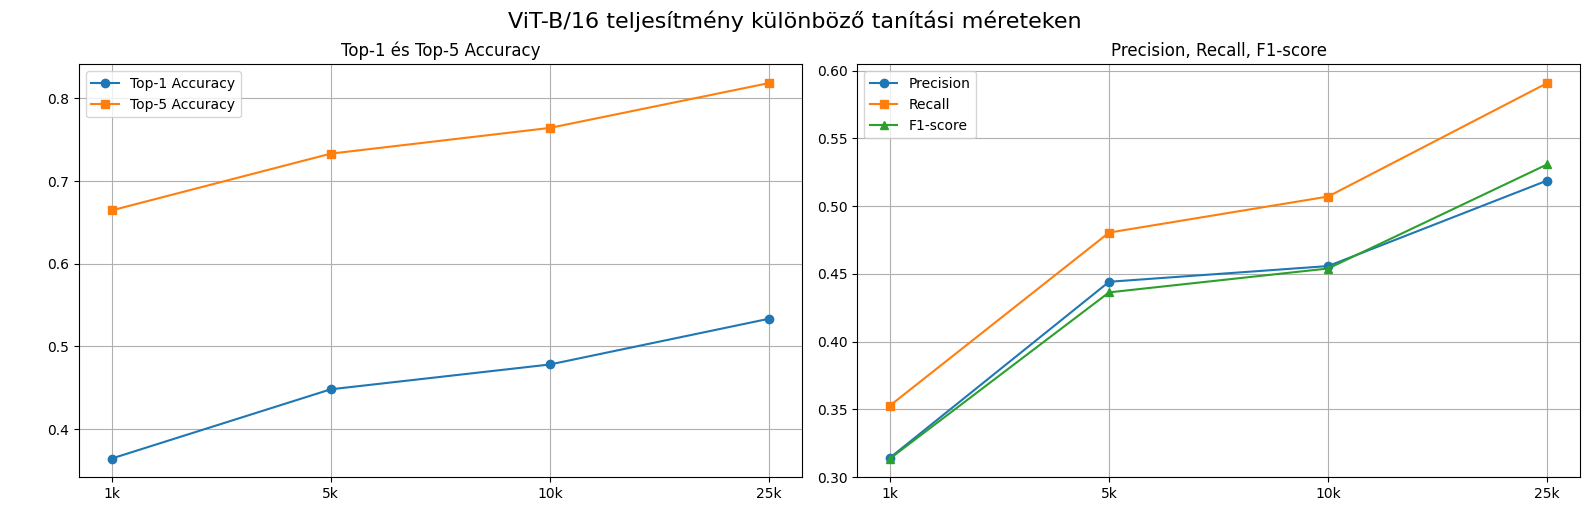
\includegraphics[width=1.0\textwidth]{images/phase03/phase03_ViT-B-16_summary_curve_metrics.png}
    \caption{Összehasonlító metrika grafikon a ViT-B-16 iteratív tanításáról.}
    \label{fig:phase03_ViT-B-16_summary_curve_metrics}
  \end{figure}

  \subsubsection{Összehasonlító idő grafikon a ViT-B-16 iteratív tanításáról.}
  \begin{figure}[H]
    \centering
    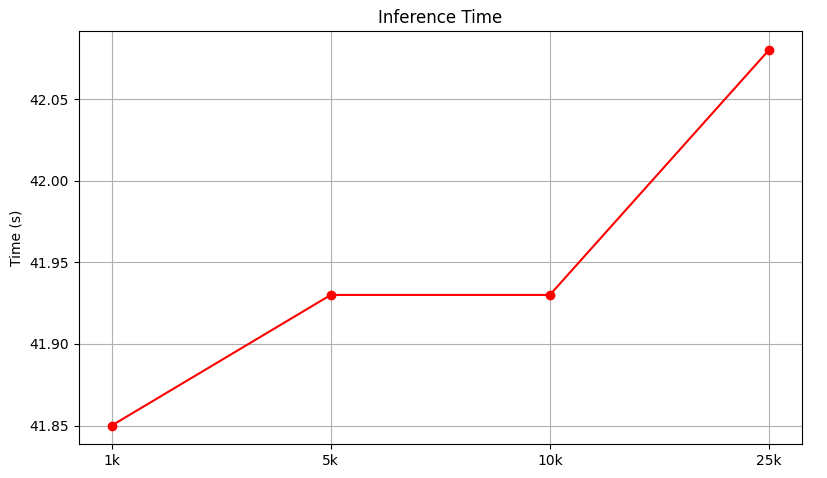
\includegraphics[width=1.0\textwidth]{images/phase03/phase03_ViT-B-16_summary_curve_time.png}
    \caption{Összehasonlító idő grafikon a ViT-B-16 iteratív tanításáról.}
    \label{fig:phase03_ViT-B-16_summary_curve_time}
  \end{figure}

  \subsubsection{Összehasonlító grafikon a ViT-B-16 iteratív tanításáról 10 EPOCH-on keresztül.}
  \begin{figure}[H]
    \centering
    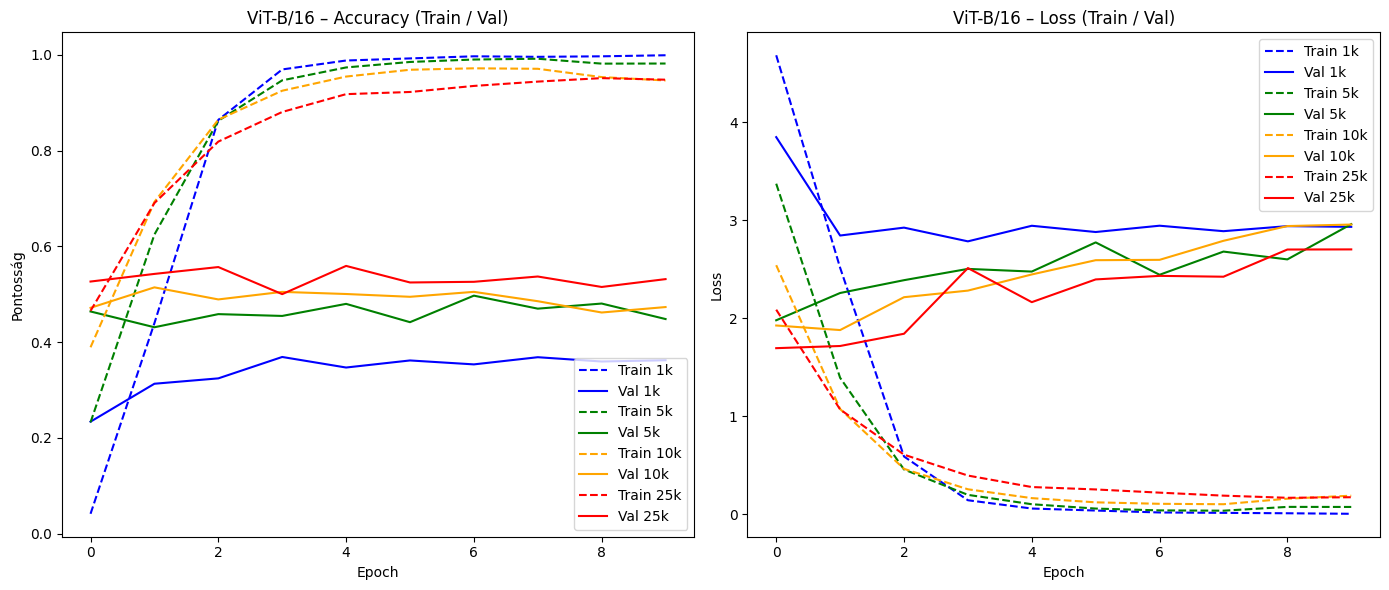
\includegraphics[width=1.0\textwidth]{images/phase03/phase03_ViT-B-16_learning_summary_curve.png}
    \caption{Összehasonlító grafikon a ViT-B-16 iteratív tanításáról 10 EPOCH-on keresztül.}
    \label{fig:phase03_ViT-B-16_learning_summary_curve}
  \end{figure}

  \subsubsection{Összehasonlító Confusion Matrix a ViT-B-16 iteratív tanításáról.}
  \begin{figure}[H]
    \centering
    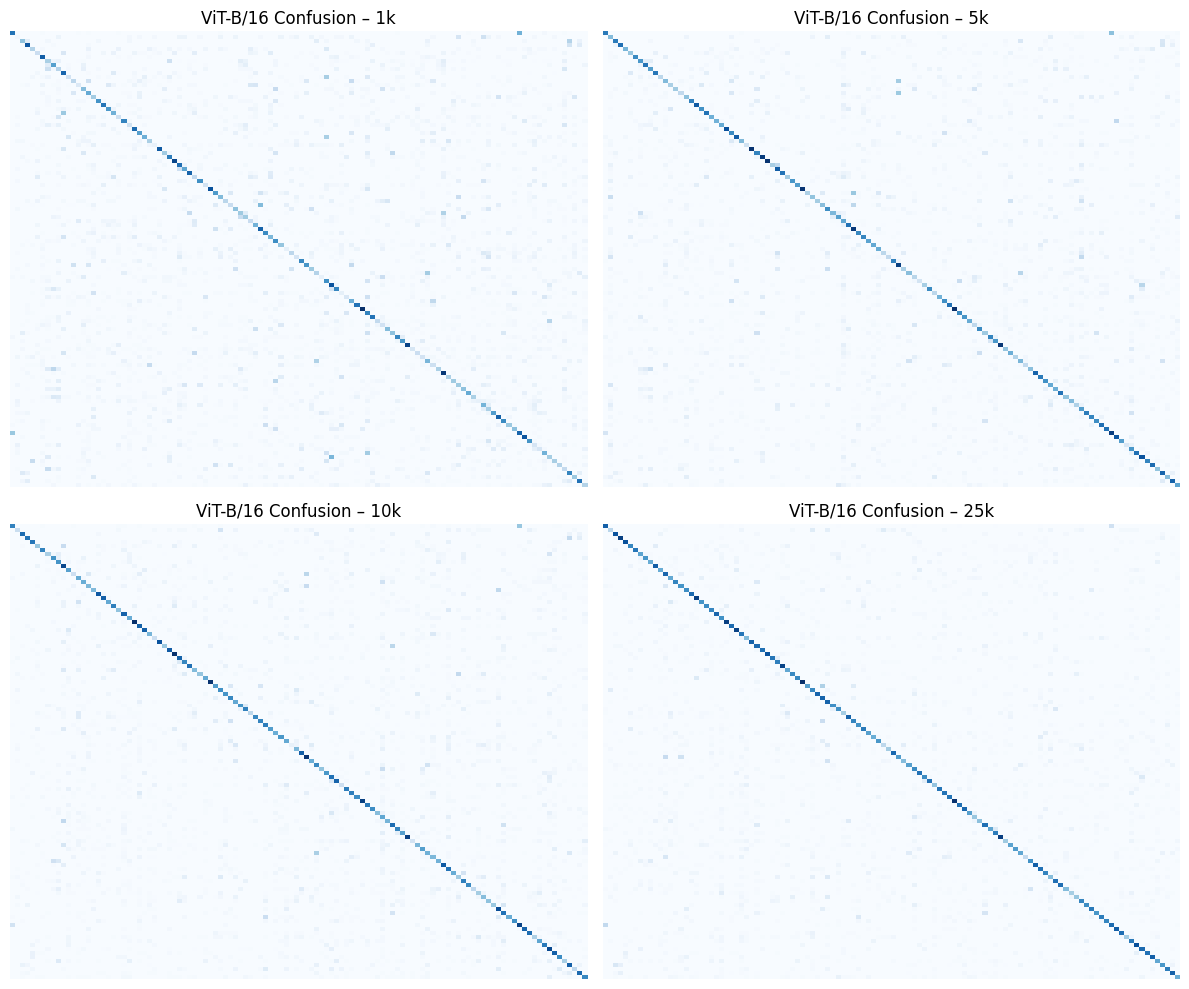
\includegraphics[width=1.0\textwidth]{images/phase03/phase03_ViT-B-16_Confusion_Matrix_summary_curve.png}
    \caption{Összehasonlító Confusion Matrix a ViT-B-16 iteratív tanításáról 10 EPOCH-on keresztül.}
    \label{fig:phase03_ViT-B-16_Confusion_Matrix_summary_curve}
  \end{figure}